%===============================================================================
% LaTeX sjabloon voor de bachelorproef toegepaste informatica aan HOGENT
% Meer info op https://github.com/HoGentTIN/latex-hogent-report
%===============================================================================

\documentclass[dutch,dit,thesis]{hogentreport}

% TODO:
% - If necessary, replace the option `dit`' with your own department!
%   Valid entries are dbo, dbt, dgz, dit, dlo, dog, dsa, soa
% - If you write your thesis in English (remark: only possible after getting
%   explicit approval!), remove the option "dutch," or replace with "english".

%% Pictures to include in the text can be put in the graphics/ folder
\graphicspath{{graphics/}}

%% For source code highlighting, requires pygments to be installed
%% Compile with the -shell-escape flag!
%\usepackage[cache=false]{minted}
\usepackage[chapter,outputdir=../output]{minted}
\usepackage{mdframed}
%% If you compile with the make_thesis.{bat,sh} script, use the following
%% import instead:
%% \usepackage[section,outputdir=../output]{minted}
\usemintedstyle{solarized-light}
\definecolor{bg}{RGB}{253,246,227} %% Set the background color of the codeframe

%% Formatting for minted environments.
\setminted{%
    autogobble,
    frame=lines,
    breaklines,
    linenos,
    tabsize=4
}

%% Ensure the list of listings is in the table of contents
\renewcommand\listoflistingscaption{%
    \IfLanguageName{dutch}{Lijst van codefragmenten}{List of listings}
}
\renewcommand\listingscaption{%
    \IfLanguageName{dutch}{Codefragment}{Listing}
}
\renewcommand*\listoflistings{%
    \cleardoublepage\phantomsection\addcontentsline{toc}{chapter}{\listoflistingscaption}%
    \listof{listing}{\listoflistingscaption}%
}

%% Change this line to edit the line numbering style:
\renewcommand{\theFancyVerbLine}{\ttfamily\scriptsize\arabic{FancyVerbLine}}

%% Macro definition to load external java source files with \javacode{filename}:
\newmintedfile[javacode]{java}{
    bgcolor=bg,
    fontfamily=tt,
    linenos=true,
    numberblanklines=true,
    numbersep=5pt,
    gobble=0,
    framesep=2mm,
    funcnamehighlighting=true,
    tabsize=4,
    obeytabs=false,
    breaklines=true,
    mathescape=false
    samepage=false,
    showspaces=false,
    showtabs =false,
    texcl=false,
}

% Other packages not already included can be imported here

%%---------- Document metadata -------------------------------------------------
\author{Maurice Cantaert}
\supervisor{Mevr. M. Van Audenrode}
\cosupervisor{Dhr. J. Van Bossuyt}
\title{Het suggereren van sportschema's door middel van objectherkenning en generatieve AI}
\academicyear{\advance\year by -1 \the\year--\advance\year by 1 \the\year}
\examperiod{1}
\degreesought{\IfLanguageName{dutch}{Professionele bachelor in de toegepaste informatica}{Bachelor of applied computer science}}
\partialthesis{false}

%% Add global exceptions to the hyphenation here
\hyphenation{back-slash}

%% The bibliography (style and settings are  found in hogentthesis.cls)
\addbibresource{bachproef.bib}            %% Bibliography file
\addbibresource{../voorstel/voorstel.bib} %% Bibliography research proposal
\defbibheading{bibempty}{}

%% Prevent empty pages for right-handed chapter starts in twoside mode
\renewcommand{\cleardoublepage}{\clearpage}

\renewcommand{\arraystretch}{1.2}

%% Content starts here.
\begin{document}

%---------- Front matter -------------------------------------------------------

\frontmatter

\hypersetup{pageanchor=false} %% Disable page numbering references
%% Render a Dutch outer title page if the main language is English
\IfLanguageName{english}{%
    %% If necessary, information can be changed here
    \degreesought{Professionele Bachelor toegepaste informatica}%
    \begin{otherlanguage}{dutch}%
       \maketitle%
    \end{otherlanguage}%
}{}

%% Generates title page content
\maketitle
\hypersetup{pageanchor=true}

%%=============================================================================
%% Voorwoord
%%=============================================================================

\chapter*{\IfLanguageName{dutch}{Woord vooraf}{Preface}}%
\label{ch:voorwoord}

%% TODO:
%% Het voorwoord is het enige deel van de bachelorproef waar je vanuit je
%% eigen standpunt (``ik-vorm'') mag schrijven. Je kan hier bv. motiveren
%% waarom jij het onderwerp wil bespreken.
%% Vergeet ook niet te bedanken wie je geholpen/gesteund/... heeft

\lipsum[1-2]
%%%=============================================================================
%% Samenvatting
%%=============================================================================

% TODO: De "abstract" of samenvatting is een kernachtige (~ 1 blz. voor een
% thesis) synthese van het document.
%
% Een goede abstract biedt een kernachtig antwoord op volgende vragen:
%
% 1. Waarover gaat de bachelorproef?
% 2. Waarom heb je er over geschreven?
% 3. Hoe heb je het onderzoek uitgevoerd?
% 4. Wat waren de resultaten? Wat blijkt uit je onderzoek?
% 5. Wat betekenen je resultaten? Wat is de relevantie voor het werkveld?
%
% Daarom bestaat een abstract uit volgende componenten:
%
% - inleiding + kaderen thema
% - probleemstelling
% - (centrale) onderzoeksvraag
% - onderzoeksdoelstelling
% - methodologie
% - resultaten (beperk tot de belangrijkste, relevant voor de onderzoeksvraag)
% - conclusies, aanbevelingen, beperkingen
%
% LET OP! Een samenvatting is GEEN voorwoord!

%%---------- Nederlandse samenvatting -----------------------------------------
%
% TODO: Als je je bachelorproef in het Engels schrijft, moet je eerst een
% Nederlandse samenvatting invoegen. Haal daarvoor onderstaande code uit
% commentaar.
% Wie zijn bachelorproef in het Nederlands schrijft, kan dit negeren, de inhoud
% wordt niet in het document ingevoegd.

\IfLanguageName{english}{%
\selectlanguage{dutch}
\chapter*{Samenvatting}
\selectlanguage{english}
}{}

%%---------- Samenvatting -----------------------------------------------------
% De samenvatting in de hoofdtaal van het document

\chapter*{\IfLanguageName{dutch}{Samenvatting}{Abstract}}
TODO

%---------- Inhoud, lijst figuren, ... -----------------------------------------

\tableofcontents

% In a list of figures, the complete caption will be included. To prevent this,
% ALWAYS add a short description in the caption!
%
%  \caption[short description]{elaborate description}
%
% If you do, only the short description will be used in the list of figures

\listoffigures

% If you included tables and/or source code listings, uncomment the appropriate
% lines.
%\listoftables
\listoflistings

% Als je een lijst van afkortingen of termen wil toevoegen, dan hoort die
% hier thuis. Gebruik bijvoorbeeld de ``glossaries'' package.
% https://www.overleaf.com/learn/latex/Glossaries

%---------- Kern ---------------------------------------------------------------

\mainmatter{}

% De eerste hoofdstukken van een bachelorproef zijn meestal een inleiding op
% het onderwerp, literatuurstudie en verantwoording methodologie.
% Aarzel niet om een meer beschrijvende titel aan deze hoofdstukken te geven of
% om bijvoorbeeld de inleiding en/of stand van zaken over meerdere hoofdstukken
% te verspreiden!

%%---------- Inleiding, stand van zaken ---------------------------------------
%%=============================================================================
%% Inleiding
%%=============================================================================

% context, achtergrond
% afbakenen van het onderwerp
% verantwoording van het onderwerp, methodologie
% probleemstelling
% onderzoeksdoelstelling
% onderzoeksvraag

\chapter{\IfLanguageName{dutch}{Inleiding}{Introduction}}
\label{ch:inleiding}
Sport kent een prominente rol in de levensstijl van Vlamingen, zo blijkt sterk in de statistieken van~\textcite{StatistiekVlaanderen2023}.
Hoewel sportparticipatie van Vlamingen hoog scoort met een gemiddelde van een op vier Vlamingen die (bijna) dagelijks een sport beoefent, kan hetzelfde niet gezegd worden over de beschikbaarheid van trainers.
Ondanks de stijging van het aantal gediplomeerde trainers blijkt in het jaarverslag van~\textcite{SportVlaanderen2023} blijkt dat sportclubs blijven kampen met een trainerstekort.
Sterker nog, het komt naar voren dat gemiddeld 26 procent van de trainers jonger dan 30 jaar afhaken, waardoor de verhouding van \'e\'en trainer op twintig sporters geen positieve evolutie kent.

Het is duidelijk dat er niet alleen werk gemaakt moet worden om meer coaches op te leiden, maar ook om tewerkgestelde trainers bij te staan in hun takenpakket.
Met de voortdurende verbeteringen binnen de artifici\"ele intelligentiesector en de toename in capaciteiten van generatieve AI ontstaan mogelijkheden om de werkdruk van trainers te verlichten.
Deze paper richt zich erop een proof-of-concept Android-app te ontwikkelen om sporters op weg te helpen met behulp van generatieve AI en objectherkenning.
Trainers kunnen vervolgens bijsturen waar nodig, waarmee de werkdruk om startende sporters bij te staan verkleind kan worden.

%%---------- Probleemstelling -------------------------------------------------
\section{\IfLanguageName{dutch}{Probleemstelling}{Problem Statement}}
\label{sec:probleemstelling}
Jordi Van Bossuyt is een jonge zelfstandige personal trainer en geeft momenteel training aan jonge cadetten in de Koninklijke Atletiekclub Eendracht Aalst.
Met een interesse voor een meer gestroomlijnde manier om startende sporters bij te staan komt het idee van een combinatie van een mobiele app met generatieve AI aan bod.
Concreet is het doel om een app te ontwikkelen waarbij er minimale frictie moet zijn om aan de slag te gaan met sportmateriaal.
Gebruikers horen de mogelijkheid te krijgen om sportgerelateerde objecten en omgevingen zoals fitnessinstrumenten of looppistes in te scannen met de camera van de telefoon en hiervoor suggesties te krijgen.
Met een proof-of-concept moet aangetoond kunnen worden dat dit mogelijk is door middel van een vooraf-getrainde dataset en bestaande generatieve AI-modellen om zelf suggestieve trainingsschema's te genereren.

%%---------- Onderzoeksvragen -------------------------------------------------
\section{\IfLanguageName{dutch}{Onderzoeksvraag}{Research question}}
\label{sec:onderzoeksvraag}
Hoe kan een bestaande kunstmatige intelligentieplatform gebruikt worden om aan objectherkenning te doen?
Kan het platform vervolgens suggesties van activiteiten voorstellen aan de gebruiker, met input van de trainer?
Op welke manier kan de trainer inspelen op het gebruik van de app?

%%---------- Onderzoeksdoelstellingen -----------------------------------------
\section{\IfLanguageName{dutch}{Onderzoeksdoelstelling}{Research objective}}
\label{sec:onderzoeksdoelstelling}
Deze bachelorproef zal zich eerst richten op het onderzoeken van de manier waarop aan objectherkenning en het suggereren van oefeningen kan gedaan worden in de vorm van een literatuurstudie.
Hierin komt tevens ook het trainen van eigen datasets aan bod om een beter begrip te krijgen op de manier waarop kunstmatige intelligentiemodellen getraind worden.
Met dit basis begrip zal een proof-of-concept uitgewerkt worden om de haalbaarheid van een mobiele app ter ondersteuning van trainers ontwikkeld kan worden.

De proof-of-concept moet hierbij voldoen aan enkele criteria van de opdrachtgever:
\begin{itemize}
    \item De app hoort op een kosteneffici\"ente manier ontwikkeld te worden, waarbij er geen vereiste is om zelf datasets te trainen.
    \item Dit moet op een beperkte, reproduceerbare, manier gebeuren voor \'e\'en fitnesstoestel.
    \item Suggesties moeten gegenereerd kunnen worden zonder de input van trainers, maar met de mogelijkheid voor trainers om deze suggesties te kunnen bijsturen.
    \item Gebruikers horen zo weinig mogelijk frictie te ervaren bij het inzenden van foto's en het ontvangen van suggesties.
\end{itemize}

%%---------- Opzet van de bachelorproef ---------------------------------------
\section{\IfLanguageName{dutch}{Opzet van deze bachelorproef}{Structure of this bachelor thesis}}
\label{sec:opzet-bachelorproef}
De rest van deze bachelorproef is als volgt opgebouwd:

In Hoofdstuk~\ref{ch:stand-van-zaken} wordt een overzicht gegeven van de stand van zaken binnen het onderzoeksdomein, op basis van een literatuurstudie.

In Hoofdstuk~\ref{ch:methodologie} wordt de methodologie toegelicht en worden de gebruikte onderzoekstechnieken besproken om een antwoord te kunnen formuleren op de onderzoeksvragen.

In Hoofdstuk~\ref{ch:shortlist} worden de gekozen technologie\"en en platformen toegelicht die gebruikt zullen worden bij het ontwikkelen van de proof-of-concept.

In Hoofdstuk~\ref{ch:proof-of-concept} wordt de uitwerking van de proof-of-concept uitgelegd samen met een demonstratie van hoe de app gebruikt kan worden.

In Hoofdstuk~\ref{ch:conclusie}, tenslotte, wordt de conclusie gegeven en een antwoord geformuleerd op de onderzoeksvragen.
Daarbij wordt ook een aanzet gegeven voor toekomstig onderzoek binnen dit domein.
\chapter{\IfLanguageName{dutch}{Stand van zaken}{State of the art}}
\label{ch:stand-van-zaken}

% Tip: Begin elk hoofdstuk met een paragraaf inleiding die beschrijft hoe
% dit hoofdstuk past binnen het geheel van de bachelorproef. Geef in het
% bijzonder aan wat de link is met het vorige en volgende hoofdstuk.

% Pas na deze inleidende paragraaf komt de eerste sectiehoofding.


%---------- Objectherkenning -----------------------------------------------------------
\section{De werking van objectherkenning}\label{sec:ls-object-detectie}
Omdat objectdetectie de kern van de proof-of-concept zal vormen, is het van essentieel belang om eerst een grondig begrip te defini\"eren van wat deze techniek precies inhoudt.
In dit hoofdstuk zal eerst computer visie aan bod komen, een van de gebieden van hedendaagse artifici\"ele intelligentie, waarbinnen objectherkenning zich plaats vindt.
Dit zal verduidelijkt worden aan de hand van enkele praktische toepassingen die vandaag al in gebruik genomen worden met behulp van computer visie en objectherkenning.
Daarna volgt een uitleg van de processen waarop beelden opgeslagen en verwerkt worden ter voorbereiding op het toepassen van objectherkenning.
Tot slot worden enkele traditionele objectdetectie algoritmen besproken die de verwerkte data kunnen interpreteren.
Met een begrip voor de verschillende stappen van computer visie en objectherkenning kan vervolgens gekeken worden naar de volgende stap die toegepast zal worden in de proof-of-concept.
Het volgende hoofdstuk in deze literatuurstudie gaat hierop verder met meer informatie rond grote taalmodellen (LLM), een ander domein binnen kunstmatige intelligentie.

\subsection{Computer visie}\label{subsec:de-kern-van-objectdetectie}
Computer visie is een van de vele vakgebieden binnen de kunstmatige intelligentie en richt zich op het interpreteren van multimedia~\autocite{Moin2023}.
Met de komst van dit vakgebied ontstaat een grote waaier aan mogelijkheden voor computers om bij te staan bij complexere taken zoals gezichts- en emotieherkenning, sc\`eneanalyse en objectherkenning.
Hiermee beschrijven~\textcite{Tasnim2023} dat objectdetectie een fundamentele taak omvat binnen dit vakgebied waarmee het identificeren en lokaliseren van objecten mogelijk wordt op (bewegende) beelden.
De ontwikkelingen in dit vakgebied worden vandaag steeds meer gebruikt in allerlei sectoren:

\subsubsection{Computer visie in de landbouwsector}
\textcite{Radojcic2023}~beschrijft in zijn conferentiepaper voor de 15de Internationale Landbouwsymposium `AGROSYM 2023' conferentie het volgende over computer visie in de landbouw:
``De integratie van robotica, slimme landbouw en computervisietechnologie\"en in de landbouw heeft een transformerende verschuiving in de industrie teweeggebracht.
Het gebruik van computervisiealgoritmen heeft een cruciale rol gespeeld in het realtime monitoren en beheren van gewassen.
Door afbeeldingen en video's te analyseren, bieden deze algoritmen boeren tijdige en nauwkeurige informatie over de groei en ontwikkeling van hun gewassen, waardoor ze ge\"{\i}nformeerde beslissingen kunnen nemen over bemesting, irrigatie en pesticidegebruik.''
Deze resultaten binnen de landbouwsector worden gerealiseerd door middel van objectherkenning binnen computervisie.
Om het gebruik hiervan mogelijk te maken worden deep learning algoritmes zoals convolutionele neurale netwerken (CNN) toegepast, meer hiervan komt aan bod in het hoofdstuk~\nameref{sec:datasets}.

\subsubsection{Computer visie in zelfrijdende auto's}
Een tweede voorbeeld is het toepassen van computer visie in de transportsector.
Met behulp van computer visie-algoritmen zoals kleurenruimte transformatie, Canny-randdetectie en Hough-lijntransformatie wordt het mogelijk voor zelfrijdende auto's om op een goedkopere wijze berekeningen te maken~\autocite{Gajjar2023}.
Door middel van deze algoritmen verdwijnt de noodzaak om te ondersteunen op duurdere systemen, met name Lichtdetectie- en afstandmetingssensoren (LiDAR) die gebruikt worden om een virtuele driedimensionele map te maken van de direct omgeving.
Beide systemen kennen een vorm van objectherkenning om objecten zoals verkeersborden of voertuigen in de omgeving te detecteren.
De implementatie hiervan kent echter de moeilijkheid van data-analyse in donkere momenten zoals na zonsondergang, waardoor de kwaliteit van binnenkomende data afzwakt door het lage licht.
Een mogelijke oplossing hierbij is het toevoegen van infrarood lampen gecombineerd met een infraroodcamera.
Ook hierbij wordt het mogelijk om via CNN-algoritmes te bepalen wanneer overgestapt moet worden op een alternatief systeem.
\begin{figure}
    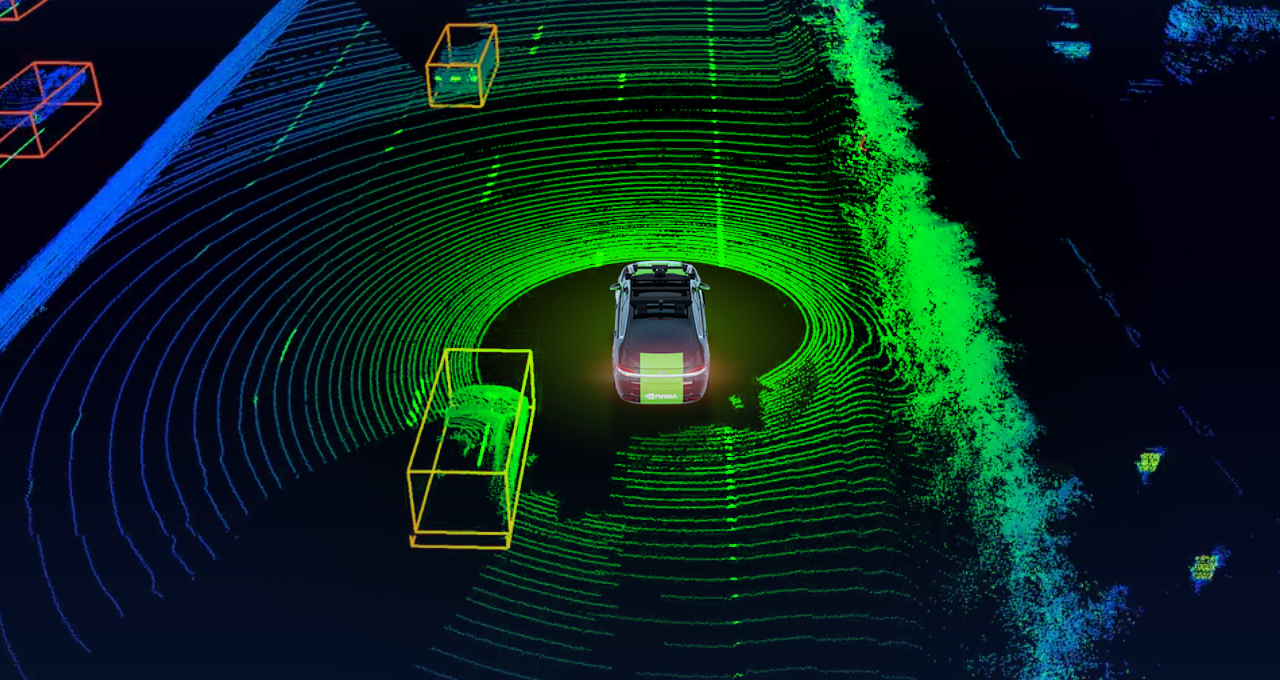
\includegraphics[width=1\linewidth]{images/visualisatie-lidar}
    \caption{Visualisatie van een LiDAR-systeem met objectherkenning in auto's~\autocite{Badoni2021}}
    \label{fig:visualisatie-lidar}
\end{figure}

\subsection{Beeldfragmenten in datavorm}\label{subsec:beeldfragmenten-als-data}
Concreet worden beelden digitaal opgeslagen in tweedimensionale tabellen van pixels, waarbij elke pixel kleurdata bevat.
De resolutie, of scherpheid, van een beeldfragment wordt vaak hierin uitgedrukt.
Zo kent een standaard Full HD (FHD)-computerscherm volgens de specificaties van~\textcite{VESA2013} een resolutie van 1920 pixels bij 1080 pixels.
Deze resolutie wordt volgens statistieken van~\textcite{ValveCorporation2024} gebruikt door meer dan de helft van haar gebruikers.
Om de kwaliteit van een beeldfragment uit te drukken wordt regelmatig gebruik gemaakt van de meeteenheid megapixels, waarbij \'e\'en megapixel \'e\'en miljoen pixels voorstelt.
Hiermee ontstaat de vaststelling dat de voorafgaande en meest gebruikte specificatie van Full HD een beeldkwaliteit van 2,1 megapixels kan weergeven aan gebruikers.

\subsubsection{Kwaliteit van hedendaags camera's}
Moderne smartphones zoals de Galaxy S24 nemen volgens~\textcite{Samsung2024} foto's aan een kwaliteit van 50 megapixels en bieden daarmee ongeveer 24 keer hogere kwaliteit dan een Full HD-computerscherm kan weergeven.
Het is hierbij belangrijk om op te merken dat het aantal megapixels niet de enige factor speelt in het bepalen van beeldkwaliteit.
Deze meeteenheid bepaalt tevens enkel de totale grootte van de data dat een beeldfragment bevat.
Ook ongewenste data, waaronder ruis en vervorming, worden hierin meegeteld.
Om dit probleem te mitigeren wordt in vele gevallen aan pixel binning gedaan, een proces waarbij pixels gegroepeerd worden tot zogenaamde superpixels~\autocite{Jin2012}.
\begin{figure}
    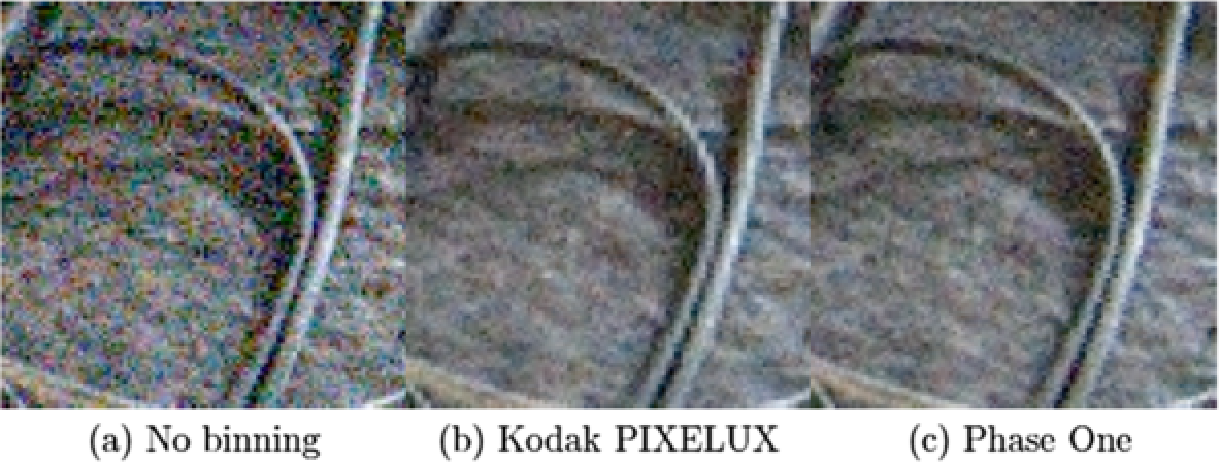
\includegraphics[width=1\linewidth]{images/pixel-binning}
    \caption{Visualisatie van pixel binning~\autocite{Jin2012}}
    \label{fig:pixel-binning}
\end{figure}

Moderne smartphones kiezen ervoor om pixels samen te nemen in groepen van vier en daarmee het binningsproces uit te voeren.
Ten gevolge van dit proces krijgen afbeeldingen een kleinere voetafdruk, wat resultaat in beelden van 12 megapixels.
Een bijkomend effect is het verzachten van observeerbare ruis waardoor beelden die genomen zijn in donkere plekken een hogere beeldkwaliteit krijgen.
De kwaliteit van beelden na het uitvoeren van dit proces liggen tussen die van de schermresoluties 4K Ultra HD (ongeveer 8 megapixels) en 8K Ultra HD (ongeveer 33 megapixels), resoluties die steeds vaker gebruikt worden in televisies~\autocite{Statista2024}.
Bovendien maakt dit het makkelijker voor computer visie-algoritmen om de gemaakte multimedia te analyseren aan een hogere nauwkeurigheid doordat er meer bruikbare data is om mee te werken.

\subsection{Het verwerken van data uit multimedia}\label{subsec:het-verwerken-van-data}
In hoofdstuk 2 van zijn onderzoek beschrijft~\textcite{Olaoye2024} het proces van beeldverwerking in enkele cruciale stappen:
% TODO: uitwerken
% beeldregistratie, filtering, segmentatie en kenmerkextractie.

\subsection{Bestaande objectherkenningsalgoritmen}\label{subsec:bestaande-algoritmen}
Na het verwerken van beeldfragmenten komt het toepassen van objectherkenning aan bod, waarvoor vele iteraties aan algoritmes geschreven zijn.
Belangrijk hierbij is om te onthouden dat elk algoritme eerst een dataset nodig heeft om te weten hoe een bepaald object eruit ziet.
Dit komt aan bod in het hoofdstuk~\nameref{sec:datasets}.
Hieronder volgen de meestgebruikte traditionele algoritmes om aan objectherkenning te doen.
Daarnaast worden enkele actuele toepassingen opgesomd en de effici\"entie van de algoritmes.

% TODO: algoritmes
\subsubsection{Algoritme A}
Algoritme A wordt uitgelegd.

% TODO: uitdagingen en beperkingen van objectdetectie
% variaties in verlichting, complexe achtergronden, schaalvariaties, vervormingen en occlusie.


%---------- De werking van AI ----------------------------------------------------------
\section{De werking van grote taalmodellen}
\label{sec:ls-artificiele-intelligentie}
In het vorig hoofdstuk kwam computer visie aan bod als vakdomein binnen de artifici\"ele intelligentie.
Een ander, en met hedendaagse coverage in het nieuws wellicht bekendere, domein hierin is de toepassing van large language models (LLM).
Voorbeelden hiervan zijn GPT en haar toepassing ChatGPT. % TODO: hier op verder gaan & kijken naar voorstel of daar niets uit genomen kan worden.

%---------- Datasets generereren ------------------------------------------------------
\section{Het trainen van datasets voor objectherkenning}\label{sec:datasets}
Uitleg hier over: % TODO
- hoe wordt bepaald wat een geldig beeld is om mee te trainen
- hoe worden datasets getraind
- misschien statistieken van hoe nauwkeurig
- bestaande datasets gebruiken zoals Google Gemini Vertex
%  populaire datasets, zoals COCO (Common Objects in Context), Pascal VOC (Visual Object Classes), en ImageNet, worden vaak gebruikt voor het trainen en evalueren van objectherkenningsalgoritmen.
%%=============================================================================
%% Methodologie
%%=============================================================================

\chapter{\IfLanguageName{dutch}{Methodologie}{Methodology}}%
\label{ch:methodologie}

%% TODO: In dit hoofstuk geef je een korte toelichting over hoe je te werk bent
%% gegaan. Verdeel je onderzoek in grote fasen, en licht in elke fase toe wat
%% de doelstelling was, welke deliverables daar uit gekomen zijn, en welke
%% onderzoeksmethoden je daarbij toegepast hebt. Verantwoord waarom je
%% op deze manier te werk gegaan bent.
%% 
%% Voorbeelden van zulke fasen zijn: literatuurstudie, opstellen van een
%% requirements-analyse, opstellen long-list (bij vergelijkende studie),
%% selectie van geschikte tools (bij vergelijkende studie, "short-list"),
%% opzetten testopstelling/PoC, uitvoeren testen en verzamelen
%% van resultaten, analyse van resultaten, ...
%%
%% !!!!! LET OP !!!!!
%%
%% Het is uitdrukkelijk NIET de bedoeling dat je het grootste deel van de corpus
%% van je bachelorproef in dit hoofstuk verwerkt! Dit hoofdstuk is eerder een
%% kort overzicht van je plan van aanpak.
%%
%% Maak voor elke fase (behalve het literatuuronderzoek) een NIEUW HOOFDSTUK aan
%% en geef het een gepaste titel.

\lipsum[21-25]



%%---------- Corpus bachelorproef ---------------------------------------------
%%=============================================================================
%% Shortlist
%%=============================================================================

\chapter{\IfLanguageName{dutch}{Selectie van tools}{Selection of tools}}
\label{ch:shortlist}
Hierna volgen enkele beslissingen rond de gebruikte tools en technologie\"en in het technische luik van deze paper.
De vereisten van de opdrachtgever staan hierbij centraal zoals besproken in de~\nameref{sec:onderzoeksdoelstelling}.
Daarnaast komt ook een korte uitleg rond de keuze voor het te testen fitnessinstrument aan bod.
Het volgende hoofdstuk beschrijft vervolgens de uitwerking van dit luik met de gekozen tools in de vorm van een proof-of-concept.

\section{Android-app met Jetpack Compose}
\label{sec:keuze-framework-voor-android-app}
TODO toelichten waarom er voor native is gekozen boven een progressive web app en crossplatform apps.

\section{Achterliggende service met Quarkus}
\label{sec:keuze-framework-voor-back-end}
TODO toelichten waarom er voor Quarkus gekozen is en wat de voordelen zijn (Quarkus Dev Services en extensies, Langchain4j, Docker/Testcontainers, Kotlin in plaats van Java).

\section{Artificiële intelligentie met Vertex AI}
\label{sec:keuze-ai-platform}
TODO toelichten waarom Google Cloud gebruikt wordt om het AI-model te hosten en waarom Google Gemini 1.5 Pro gekozen werd als model.

\section{Build tool}
\label{sec:build-tool}
Moderne software projecten maken tegenwoordig gebruik van een \textit{build tool}, wat helpt bij vele taken binnen het ontwikkelingsproces.
Bovendien is dit een vereiste voor complexere applicaties waar enkele tussenstappen vereist zijn, zoals bij het bouwen van een Android-applicatie.
Eveneens vergemakkelijkt het gebruik van een bouwsysteem om de proof-of-concept reproduceerbaar te houden.

\subsection{Motivering}
\label{subsec:voordelen-van-een-build-tool}
\textcite{Kandhway2019}~beschrijven de vijf grootste voordelen van het gebruiken van een build tool:
\begin{itemize}
    \item \textbf{Het automatiseert het bouwproces van software.}
    Software moet eerst gecompileerd worden om leesbaar en uitvoerbaar te zijn door een machine.
    Dit is automatiseerbaar aan de hand van een build tool, wat zal helpen bij het~\nameref{subsec:reproduceren-van-de-proof-of-concept}.
    \item \textbf{Het vergemakkelijkt het beheren van afhankelijkheden.}
    De achterliggende Quarkus service en de Android app zullen gebruik maken van libraries om het ontwikkelingsproces te vereenvoudigen.
    Een voorbeeld hiervan is het gebruik van de Quarkus REST-extensie, wat het verwerken van appgebruikers' verzoeken versoepelt.
    \item \textbf{Het verzekert het correct uitvoeren van het bouwproces.}
    Het bouwproces bestaat uit verschillende stappen die ondergaan moeten worden.
    Een build tool helpt hierbij om sommige stappen voor ons te bepalen, zoals de volgorde waarin afhankelijkheden inladen.
    \item \textbf{Het bespaart tijd door taken in parallel uit te voeren.}
    De build tool splitst taken op om gelijktijdig uit te voeren.
    Dit versnelt het bouwproces.
    \item \textbf{Het is een vereiste voor het toepassen van continuous integration.}
    \textit{Continuous integration} maakt het mogelijk om vooraf gedefinieerde bouwprocessen te lanceren eens er nieuwe code beschikbaar komt.
\end{itemize}

\subsection{Gradle}
\label{subsec:gradle}
Binnen het Java-ecosysteem staan Apache Maven en Gradle centraal als build tools.
Bij sommige oudere applicaties is het Ant-bouwsysteem nog in gebruik.
Het Kotlin-ecosysteem kent de voorkeur naar Maven en Gradle gezien haar oorspronkelijk ontwerp om interoperabiliteit met Java te verzekeren.
Google, de ontwikkelaars achter het Jetpack Compose framework en het Android besturingssysteem, hebben ervoor gekozen om uitsluitend met Gradle te werken wegens de beperktheid van Maven op vlak van bouwprocessen opstellen.
Met de keuze voor Jetpack Compose zoals besproken in~\ref{sec:keuze-framework-voor-android-app} zal daarmee ook gebruik gemaakt worden van Gradle voor de achterliggende Quarkus service.
De reden hiervoor is om het bouwproces zo gestroomlijnd en consistent mogelijk te houden tussen de te ontwikkelende platformen, de visualisatie van dit bouwproces is te zien in~\ref{fig:visualisatie-gradle-bouwproces}.
Een bijkomend voordeel is de mogelijkheid om de Kotlin-syntax te gebruiken binnen Gradlebestanden.
\begin{figure}
    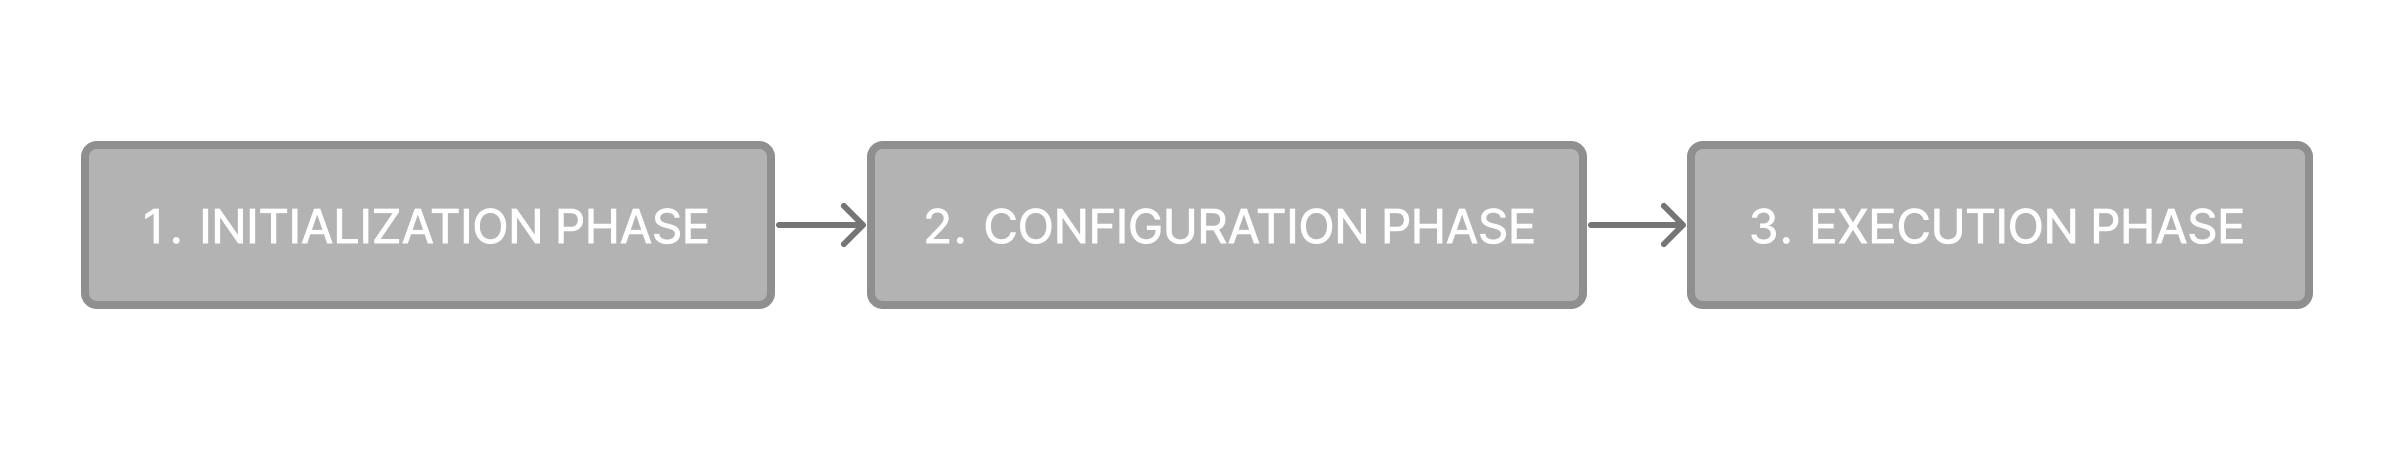
\includegraphics[width=1\linewidth]{images/gradle-buildprocess}
    \caption{De drie stappen in het Gradle bouwproces~\autocite{Gradle}}
    \label{fig:visualisatie-gradle-bouwproces}
\end{figure}

\section{Gekozen fitnessinstrument}
\label{sec:gekozen-fitnessinstrument}
TODO criteria voor het gekozen fitness instrument dat getest moest worden met motivering
%%=============================================================================
%% Proof of Concept
%%=============================================================================

\chapter{\IfLanguageName{dutch}{Proof-of-concept}{Proof-of-concept}}
\label{ch:proof-of-concept}
Na de~\nameref{ch:shortlist} kan de proof-of-concept uitgewerkt worden.
Allereerst worden de omgevingen opgezet om het uitwerken van de proof-of-concept mogelijk te maken.
Hierna komt het schrijven van de logica achter de app en achterliggende service aan bod.
Ten slotte worden enkele belangrijke details rond reproduceerbaarheid aangehaald.

De uitgewerkte broncode kan teruggevonden worden in deze GitHub repository(TODO). % TODO github url

\section{Omgevingen opzetten}
\label{sec:omgevingen-opzetten}
De drie lagen van de~\nameref{subsubsec:architectuur} kennen enkele configuratiestappen tijdens het opzetten, de documentatie daarvan volgt hieronder.

\subsection{Opzetten Google Gemini omgeving}
\label{subsec:opzetten-google-gemini-omgeving}
%Hier wordt het AI-platform opgezet om objectherkenning en suggereren van fitnessschema's mogelijk te maken TODO
TODO

\subsection{Opzetten Quarkus service}
\label{subsec:opzetten-quarkus-service}
De achterliggende service zal gebruik maken van de ingebouwde Quarkus extensies en Dev Services, zoals gezien in hoofdstuk~\ref{ch:shortlist}.
Hoewel Quarkus vele taken voor de ontwikkelaar vergemakkelijkt vergt het enigszins wat opzetwerk.

\subsubsection{Quarkus met Kotlin/Gradle}
%Opzetten Quarkus project met Kotlin en extensies TODO
TODO

\subsubsection{Testcontainers en Docker}
%Opzetten test containers met configuratie TODO
TODO

\subsection{Opzetten Jetpack Compose Android-app}
\label{subsec:opzetten-jetpack-compose-android-app}
TODO % TODO

\subsection{Reproduceren van de proof-of-concept}
\label{subsec:reproduceren-van-de-proof-of-concept}
%Uitleggen waarom dit belangrijk is (zie cursus RM) TODO
TODO

\subsubsection{Gebruikte hardware en software}
TODO % TODO

\subsubsection{Automatisatie script}
%Docker script, jar file vanuit gradle builden enz TODO
TODO

%%%=============================================================================
%% Conclusie
%%=============================================================================

\chapter{Conclusie}%
\label{ch:conclusie}
Conclusie trekken.

% TODO: Trek een duidelijke conclusie, in de vorm van een antwoord op de
% onderzoeksvra(a)g(en). Wat was jouw bijdrage aan het onderzoeksdomein en
% hoe biedt dit meerwaarde aan het vakgebied/doelgroep? 
% Reflecteer kritisch over het resultaat. In Engelse teksten wordt deze sectie
% ``Discussion'' genoemd. Had je deze uitkomst verwacht? Zijn er zaken die nog
% niet duidelijk zijn?
% Heeft het onderzoek geleid tot nieuwe vragen die uitnodigen tot verder 
%onderzoek?
 TODO

%---------- Bijlagen -----------------------------------------------------------

\appendix

\chapter{Onderzoeksvoorstel}

Het onderwerp van deze bachelorproef is gebaseerd op een onderzoeksvoorstel dat vooraf werd beoordeeld door de promotor. Dat voorstel is opgenomen in deze bijlage.

\section*{Samenvatting}

% Kopieer en plak hier de samenvatting (abstract) van je onderzoeksvoorstel.

% Verwijzing naar het bestand met de inhoud van het onderzoeksvoorstel
%%---------- Inleiding ---------------------------------------------------------

\section{Introductie}%
\label{sec:introductie}

Augmented reality, of kortweg AR, omvat een samensmelting van de virtuele wereld met de echte wereld door middel van een overlay.
Met haar eerste iteratie in de vorm van een head-mounted display ontwikkeld door \textcite{Sutherland1968} , kende deze technologie een opmerkelijke voorsprong op de hedendaagse smartphone.
Toch kent deze vorm van AR niet dezelfde aanneming door het algemene publiek en is tot recentelijk enkel een vorm van mobiele AR (gebruikmakend van smartphones) aanwezig op de markt.

Head-mounted AR had vooral te lijden aan grotere technologische obstakels waaronder de displays van het apparaat zelf. \autocite{YunHan2018}
Hierdoor was het aan koplopers zoals Meta en Varjo om aanzienlijke budgetten te besteden om deze obstakels te kunnen overbruggen en de fundamenten van deze markt tot stand te krijgen.
Eerst kwamen zakelijke modellen zoals de Meta Quest Pro en Varjo XR-1, gevolgd door een influx aan consument-gerichte versies waaronder de Meta Quest 3 en de opkomende Apple VisionPro.

Tropos AR biedt een out of the box user interface (UI) aan voor mobiele AR-ontwikkelaars via haar Troposphere software-development kit.
Ontwikkelaars hoeven hierdoor niet langer te focussen op de UI, een groot onderdeel van wat mobiele AR maakt wat het is, waardoor ontwikkelingstijd aanzienlijk verkleind kan worden.
Echter, met de komst van steeds vaker gekochte consument-gerichte AR-apparaten ontstaat een nieuwe markt voor AR-ontwikkelaars.
Hoewel Tropos AR reeds knowhow opgebouwd heeft van bestaande UI-technieken binnen AR op smartphones, kunnen deze niet altijd even goed vertaald worden naar head-mounted AR.

Concreet is Tropos AR op zoek naar een nieuwe, meer intu\"{\i}tieve manier van interageren met de virtuele objecten die via AR in de echte wereld geprojecteerd worden.
Ook is er vraag naar de verschillende manieren om een menu af te beelden en hierbinnen te navigeren.
Uit dit onderzoek zal een rapport met aanbevelingen ontstaan voor Tropos AR.


%---------- Stand van zaken ---------------------------------------------------

\section{State-of-the-art}%
\label{sec:state-of-the-art}

Hier beschrijf je de \emph{state-of-the-art} rondom je gekozen onderzoeksdomein, d.w.z.\ een inleidende, doorlopende tekst over het onderzoeksdomein van je bachelorproef. Je steunt daarbij heel sterk op de professionele \emph{vakliteratuur}, en niet zozeer op populariserende teksten voor een breed publiek. Wat is de huidige stand van zaken in dit domein, en wat zijn nog eventuele open vragen (die misschien de aanleiding waren tot je onderzoeksvraag!)?

Je mag de titel van deze sectie ook aanpassen (literatuurstudie, stand van zaken, enz.). Zijn er al gelijkaardige onderzoeken gevoerd? Wat concluderen ze? Wat is het verschil met jouw onderzoek?

Verwijs bij elke introductie van een term of bewering over het domein naar de vakliteratuur, bijvoorbeeld~\autocite{Sutherland1968}! Denk zeker goed na welke werken je refereert en waarom.

Draag zorg voor correcte literatuurverwijzingen! Een bronvermelding hoort thuis \emph{binnen} de zin waar je je op die bron baseert, dus niet er buiten! Maak meteen een verwijzing als je gebruik maakt van een bron. Doe dit dus \emph{niet} aan het einde van een lange paragraaf. Baseer nooit teveel aansluitende tekst op eenzelfde bron.

Als je informatie over bronnen verzamelt in JabRef, zorg er dan voor dat alle nodige info aanwezig is om de bron terug te vinden (zoals uitvoerig besproken in de lessen Research Methods).

% Voor literatuurverwijzingen zijn er twee belangrijke commando's:
% \autocite{KEY} => (Auteur, jaartal) Gebruik dit als de naam van de auteur
%   geen onderdeel is van de zin.
% \textcite{KEY} => Auteur (jaartal)  Gebruik dit als de auteursnaam wel een
%   functie heeft in de zin (bv. ``Uit onderzoek door Doll & Hill (1954) bleek
%   ...'')

Je mag deze sectie nog verder onderverdelen in subsecties als dit de structuur van de tekst kan verduidelijken.

%---------- Methodologie ------------------------------------------------------
\section{Methodologie}%
\label{sec:methodologie}

Hier beschrijf je hoe je van plan bent het onderzoek te voeren. Welke onderzoekstechniek ga je toepassen om elk van je onderzoeksvragen te beantwoorden? Gebruik je hiervoor literatuurstudie, interviews met belanghebbenden (bv.~voor requirements-analyse), experimenten, simulaties, vergelijkende studie, risico-analyse, PoC, \ldots?

Valt je onderwerp onder één van de typische soorten bachelorproeven die besproken zijn in de lessen Research Methods (bv.\ vergelijkende studie of risico-analyse)? Zorg er dan ook voor dat we duidelijk de verschillende stappen terug vinden die we verwachten in dit soort onderzoek!

Vermijd onderzoekstechnieken die geen objectieve, meetbare resultaten kunnen opleveren. Enquêtes, bijvoorbeeld, zijn voor een bachelorproef informatica meestal \textbf{niet geschikt}. De antwoorden zijn eerder meningen dan feiten en in de praktijk blijkt het ook bijzonder moeilijk om voldoende respondenten te vinden. Studenten die een enquête willen voeren, hebben meestal ook geen goede definitie van de populatie, waardoor ook niet kan aangetoond worden dat eventuele resultaten representatief zijn.

Uit dit onderdeel moet duidelijk naar voor komen dat je bachelorproef ook technisch voldoen\-de diepgang zal bevatten. Het zou niet kloppen als een bachelorproef informatica ook door bv.\ een student marketing zou kunnen uitgevoerd worden.

Je beschrijft ook al welke tools (hardware, software, diensten, \ldots) je denkt hiervoor te gebruiken of te ontwikkelen.

Probeer ook een tijdschatting te maken. Hoe lang zal je met elke fase van je onderzoek bezig zijn en wat zijn de concrete \emph{deliverables} in elke fase?

%---------- Verwachte resultaten ----------------------------------------------
\section{Verwacht resultaat, conclusie}%
\label{sec:verwachte_resultaten}

Hier beschrijf je welke resultaten je verwacht. Als je metingen en simulaties uitvoert, kan je hier al mock-ups maken van de grafieken samen met de verwachte conclusies. Benoem zeker al je assen en de onderdelen van de grafiek die je gaat gebruiken. Dit zorgt ervoor dat je concreet weet welk soort data je moet verzamelen en hoe je die moet meten.

Wat heeft de doelgroep van je onderzoek aan het resultaat? Op welke manier zorgt jouw bachelorproef voor een meerwaarde?

Hier beschrijf je wat je verwacht uit je onderzoek, met de motivatie waarom. Het is \textbf{niet} erg indien uit je onderzoek andere resultaten en conclusies vloeien dan dat je hier beschrijft: het is dan juist interessant om te onderzoeken waarom jouw hypothesen niet overeenkomen met de resultaten.

 TODO

%%---------- Andere bijlagen --------------------------------------------------
% TODO: Voeg hier eventuele andere bijlagen toe. Bv. als je deze BP voor de
% tweede keer indient, een overzicht van de verbeteringen t.o.v. het origineel.
%\input{...}

%%---------- Backmatter, referentielijst ---------------------------------------

\backmatter{}

\setlength\bibitemsep{2pt} %% Add Some space between the bibliograpy entries
\printbibliography[heading=bibintoc]

\end{document}
